% source: https://git.fslab.de/mmklab/latex-templates/tree/master/presentation

\documentclass{beamer}

%\useoutertheme{progress}

\usepackage{etoolbox}
\newtoggle{german}

% % % % % LANGUAGE % % % %
% Make your choice here
\togglefalse{german} % English
%\toggletrue{german} % German
% % % % % \LANGUAGE % % % %

% % % Handouts % % %
%\usepackage{handoutWithNotes}
%\pgfpagesuselayout{2 on 1 with notes landscape}[a4paper,border shrink=5mm]
% % % Handouts % % %


\iftoggle{german}{
\usepackage[ngerman]{babel} % Deutsche Sprachanpassungen
\usepackage[T1]{fontenc}    % Silbentrennung bei Sonderzeichen
\usepackage[utf8]{inputenc} % Direkte Angabe von Umlauten im Dokument.Wenn Sie an einem Mac sitzen,verwenden Sie ggf. „macce“ anstatt „utf8“.
\usepackage[autostyle=true,german=quotes]{csquotes} % Anfuehrungszeichen\
}{
\usepackage[utf8]{inputenc}}


\usepackage[utf8]{inputenc}
\usepackage[T1]{fontenc}
\usepackage{textcomp}
\setbeamercovered{transparent}
\usepackage{default}
\usepackage{lmodern}
\usepackage{amsmath,amsfonts,amssymb} % Mathe
\usepackage{eurosym}
\usepackage{tikz}
\usepackage{graphicx}
%\usepackage[labelformat=empty]{caption}
\usepackage{verbatim}
\usepackage{color}
\usepackage{hypernat}
\usepackage{tabularx}
\usepackage[]{units}
\usepackage{caption}
\usepackage{comment}
%\usepackage{subfigure}
\usepackage{wasysym}
\usepackage{ulem}
\usepackage[printonlyused]{acronym} 
\usepackage{tabularx}
\usepackage{appendixnumberbeamer}
\usepackage{epigraph}
\usepackage{remreset}% tiny package containing just the \@removefromreset command
\usepackage{subcaption}
\usepackage{makecell}
\usepackage{pdfpcnotes}% Usefull package for notes for presentations
\usepackage{colorbar}
%\usepackage{./progbar}
%\usepackage{./beamerouterthemeprogress}

\let\Tiny=\tiny % Reduces a few recent error on Unix systems

\usepackage[sorting=none,style=numeric-comp,backend=bibtex,firstinits=true]{biblatex} % load the package
\addbibresource{./bibliography.bib} % Add your bib file
\renewcommand*{\bibfont}{\footnotesize}

% % % % Style % % % %
% Some colours as used in other programms like openoffice
\definecolor{red}{RGB}{184,71,71}
\definecolor{green}{RGB}{51,204,102}
\definecolor{blue}{RGB}{0,153,255}
\definecolor{fhblau}{rgb}{0, 0.594, 0.949}

\setbeamercolor{title}{bg=fhblau, fg=white}
\setbeamercolor{frametitle}{bg=fhblau, fg=white}
\setbeamercolor{structure}{fg=fhblau}

% MISC Styles %
\setbeamertemplate{bibliography item}[text]
\usetheme{default}
\setbeamertemplate{footline}[frame number]
\setbeamertemplate{caption}[numbered]
\setbeamersize{text margin left=0.3cm,text margin right=0.3cm}
\setbeamertemplate{navigation symbols}{}%remove navigation symbols
\makeatletter
\@removefromreset{subsection}{section}
\makeatother
\setcounter{subsection}{1}


% Here are some usefulf different fonts. Use them in every flooting enviroment with \usebeamerfont{AAA}
\setbeamerfont{AAA}{size*={16.00}{15.00}}
\setbeamerfont{aaa}{size*={12.00}{11.00}}
\setbeamerfont{bbb}{size*={11.00}{11.00}}
\setbeamerfont{ccc}{size*={10.00}{11.00}}
\setbeamerfont{ddd}{size*={9.00}{11.00}}
\setbeamerfont{eee}{size*={8.00}{11.00}}
\setbeamerfont{fff}{size*={7.75}{10.75}}
\setbeamerfont{ggg}{size*={7.50}{10.50}}
\setbeamerfont{hhh}{size*={7.25}{10.25}}
\setbeamerfont{iii}{size*={7.00}{10.00}}
\setbeamerfont{jjj}{size*={6.00}{9.00}}
\setbeamerfont{kkk}{size*={5.00}{8.00}}
\setbeamerfont{lll}{size*={4.00}{7.00}}
\setbeamerfont{mmm}{size*={3.00}{6.00}}
\setbeamerfont{nnn}{size*={2.00}{5.00}} 

% Set some beamer fonts
\setbeamerfont{title}{size=\Large,series=\bfseries,parent=structure}
\setbeamerfont{caption}{size=\footnotesize}
\setbeamertemplate{footline}[text line]{%
	\parbox{\linewidth}{\vspace*{-8pt}\hspace{1em}\insertshortauthor\hspace{8mm} Sematic Segmentation using Resource Efficient Deep Learning \hfill\insertpagenumber/\inserttotalframenumber}}

\renewcommand*{\bibfont}{\usebeamerfont{kkk}}

% A new cell type
\newcommand{\specialcell}[2][c]{%
  \begin{tabular}[#1]{@{}c@{}}#2\end{tabular}}

% This is usefull if you want to use enumerations over several frames
\newcounter{saveenumi}
\newcommand{\seti}{\setcounter{saveenumi}{\value{enumi}}}
\newcommand{\conti}{\setcounter{enumi}{\value{saveenumi}}}

% logo of my university
\titlegraphic{
\centering %
\includegraphics[height=1.5cm]{./logos/logo_hbrs.png} \hspace{2cm} % For external companies

\includegraphics[height=1.5cm]{./logos/logo_hbrs.png}}


% % % % % Opening % % % %
\title[]{Sematic Segmentation using\\ Resource Efficient Deep Learning}
\author[Naresh Kumar Gurulingan]{Naresh Kumar Gurulingan, Deebul Nair, Paul G. Pl\"oger}
\date{\today}
\institute[HBRS]{Hochschule Bonn-Rhein-Sieg}
\def\ThesisPubDate{\today} % Change here to the date you are going to print your thesis
\subject{Sematic Segmentation using Resource Efficient Deep Learning}
\keywords{}


\begin{document}

% Title Frame
\begin{frame}
\pnote{Here are some nodes. They are not visible on the first slides} % Notes
\titlepage
\end{frame}

\iftoggle{german}{
\begin{frame}{Agenda}
\usebeamerfont{ccc}
\tableofcontents
\end{frame}
}{
\begin{frame}{Table of Contents}
\usebeamerfont{ccc}
\tableofcontents
\end{frame}
}

\section{Introduction}
% First Frame
\begin{frame}{Introduction}

	\textbf{Semantic segmentation}
	
	Divide an input image into different regions which contain a desired object or background.
	
	\begin{figure}[!htb]
		\centering
		
\includegraphics[width=.6\linewidth]{images/em_01_023}
		\caption{Left: Input image; Right: Segmentation result.}
		\label{Fig:real}
	\end{figure}

\end{frame}

\section{Applications}
% First Frame
\begin{frame}{Applications}
	\begin{itemize}
  \item[a] {
    Autonomous cars
  }
  \item[b] {
    Robotics
  }
  \item[c] {
    Augmented reality
  }
  \end{itemize}
  
  \begin{figure}
		\begin{subfigure}{0.3\textwidth}
			\centering
			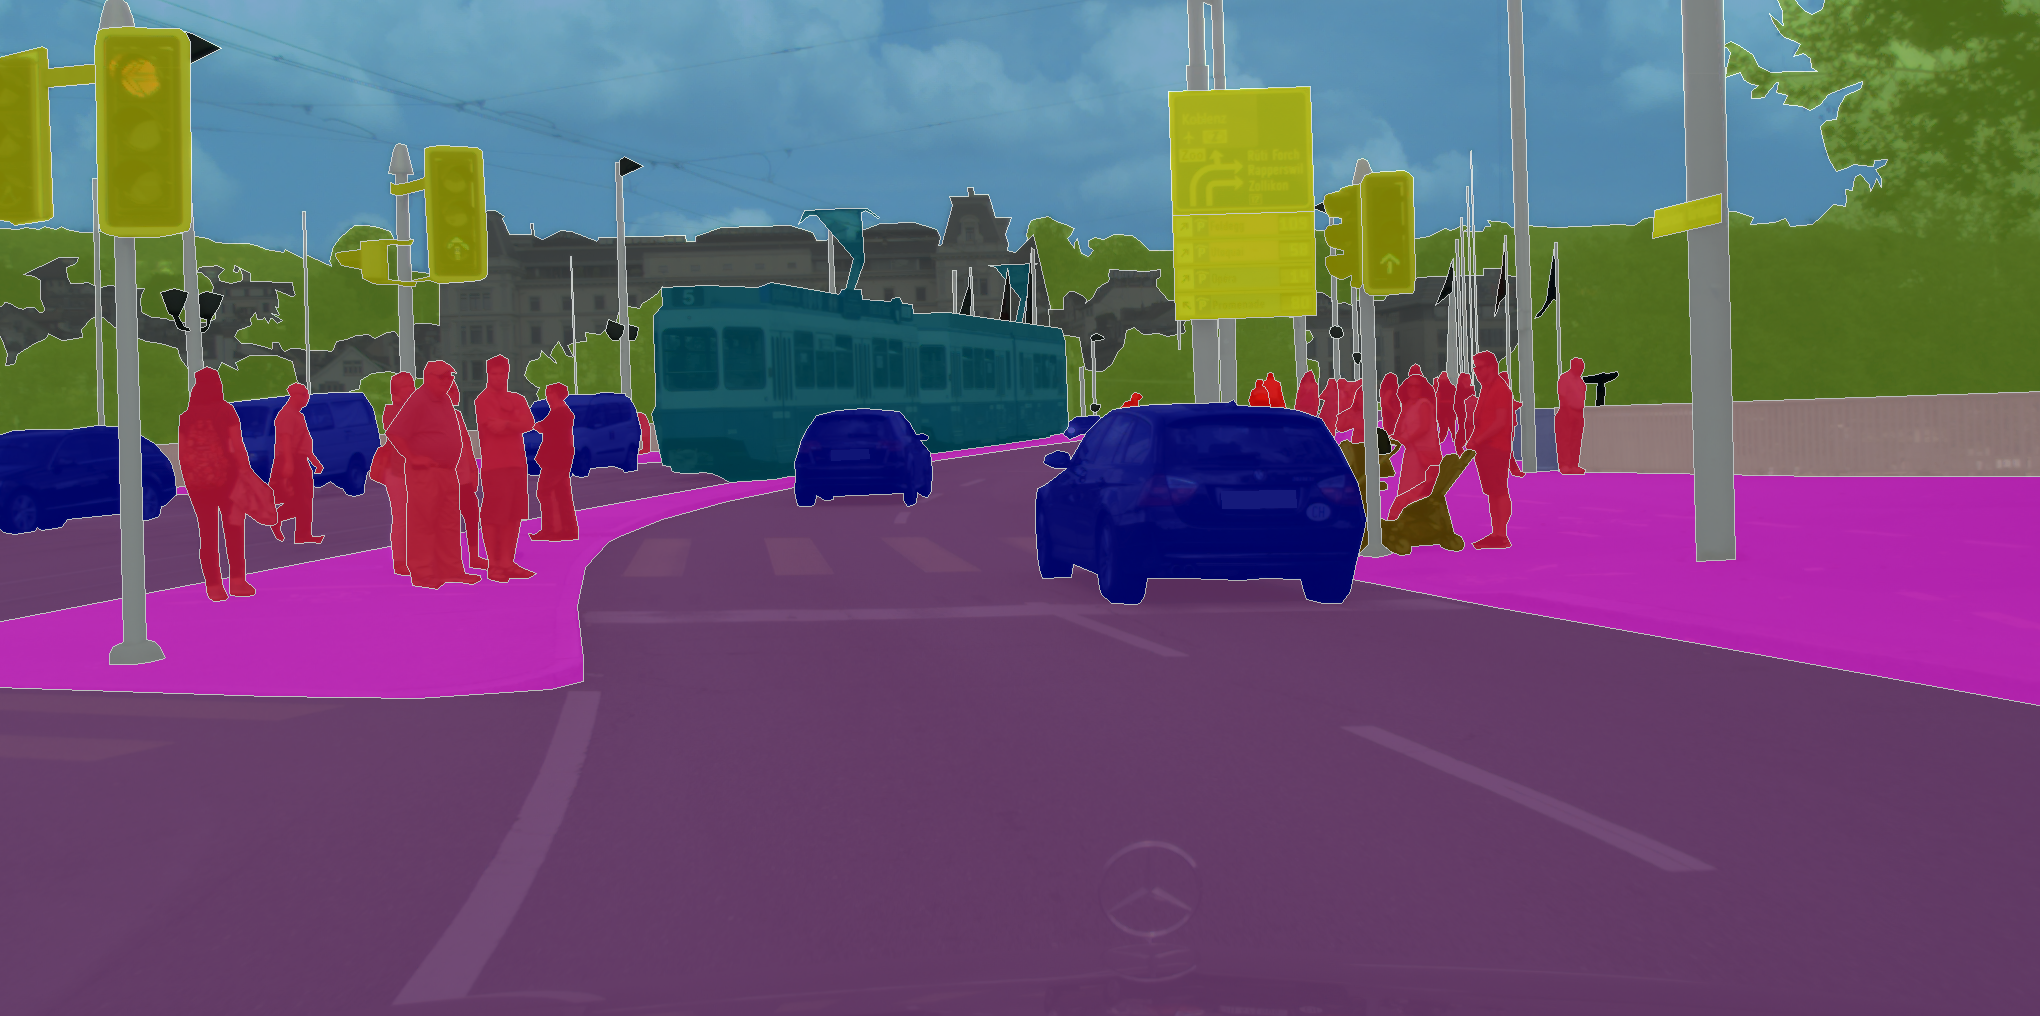
\includegraphics[width=0.95\linewidth]{images/auto_driving}
			\captionsetup{justification=centering,margin=0.2cm}
			\caption{Street scene \cite{cityscapes}}
		\end{subfigure}
		\begin{subfigure}{0.3\textwidth}
			\centering
			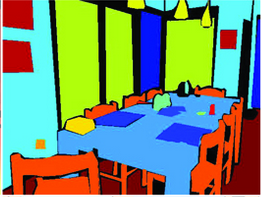
\includegraphics[width=0.8\linewidth]{images/indoor}
			\captionsetup{justification=centering,margin=0.2cm}
			\caption{Indoor scene \cite{indoor}}
		\end{subfigure}
		\begin{subfigure}{0.3\textwidth}
			\centering
			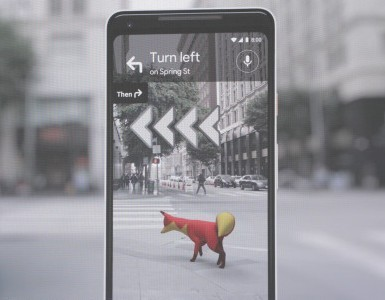
\includegraphics[width=0.8\linewidth]{images/vr_dog}
			\captionsetup{justification=centering,margin=0.2cm}
			\caption{Augmented guide \cite{techcrunch}}
		\end{subfigure}
		%\caption{(a)Street scene, (b) Indoor scene, (c) Augmented guide.}
		\label{Fig:app}
	\end{figure}

\end{frame}

\section{Dataset}

\begin{frame}{Dataset}
	
	\textbf{Objects in the dataset}
	\begin{small}
		\begin{itemize}
			\item First row from left: distance\_tube, m20, bearing, axis, r20, m30, m20\_100, motor, bearing\_box\_ax16, bearing\_box\_ax01, f20\_20\_B, f20\_20\_G. 
			\item Second row from left: em\_01, s40\_40\_B, s40\_40\_G, em\_02, container\_box\_red, container\_box\_blue.
		\end{itemize}
	\end{small}
	\begin{figure}[h]
		\centering
		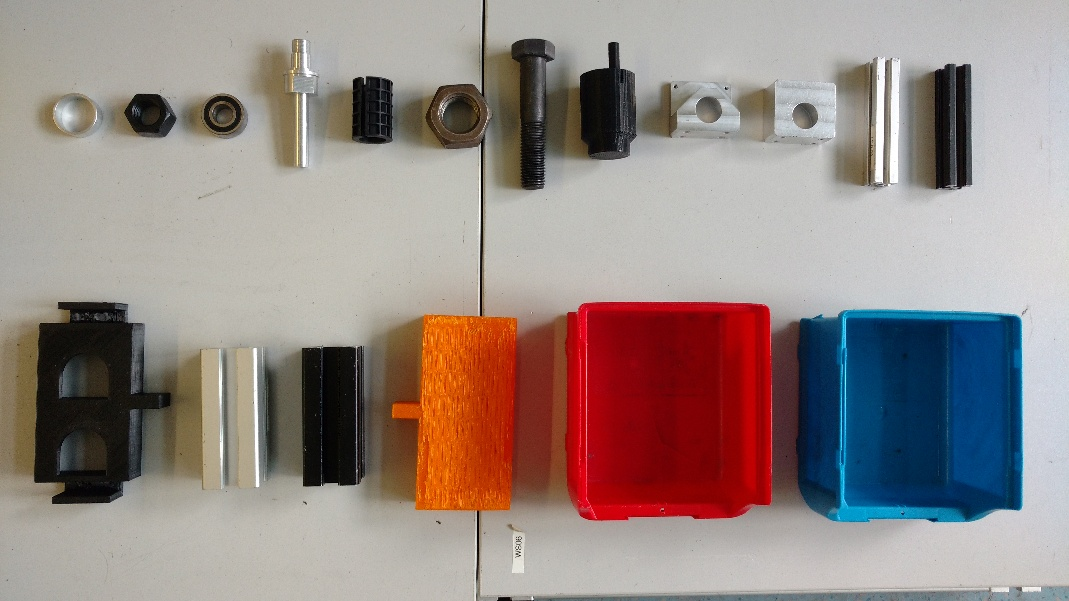
\includegraphics[scale=0.2]{images/all_objects}
		\captionsetup{justification=centering,margin=0.2cm}
		\caption{18 objects in the dataset.}
		\label{Fig:allobjects}
	\end{figure}

\end{frame}

\section{Annotation process}

\begin{frame}{Annotation process}
	
	\textbf{MATLAB ImageLabeler}
	\begin{figure}[!htb]
		\centering
		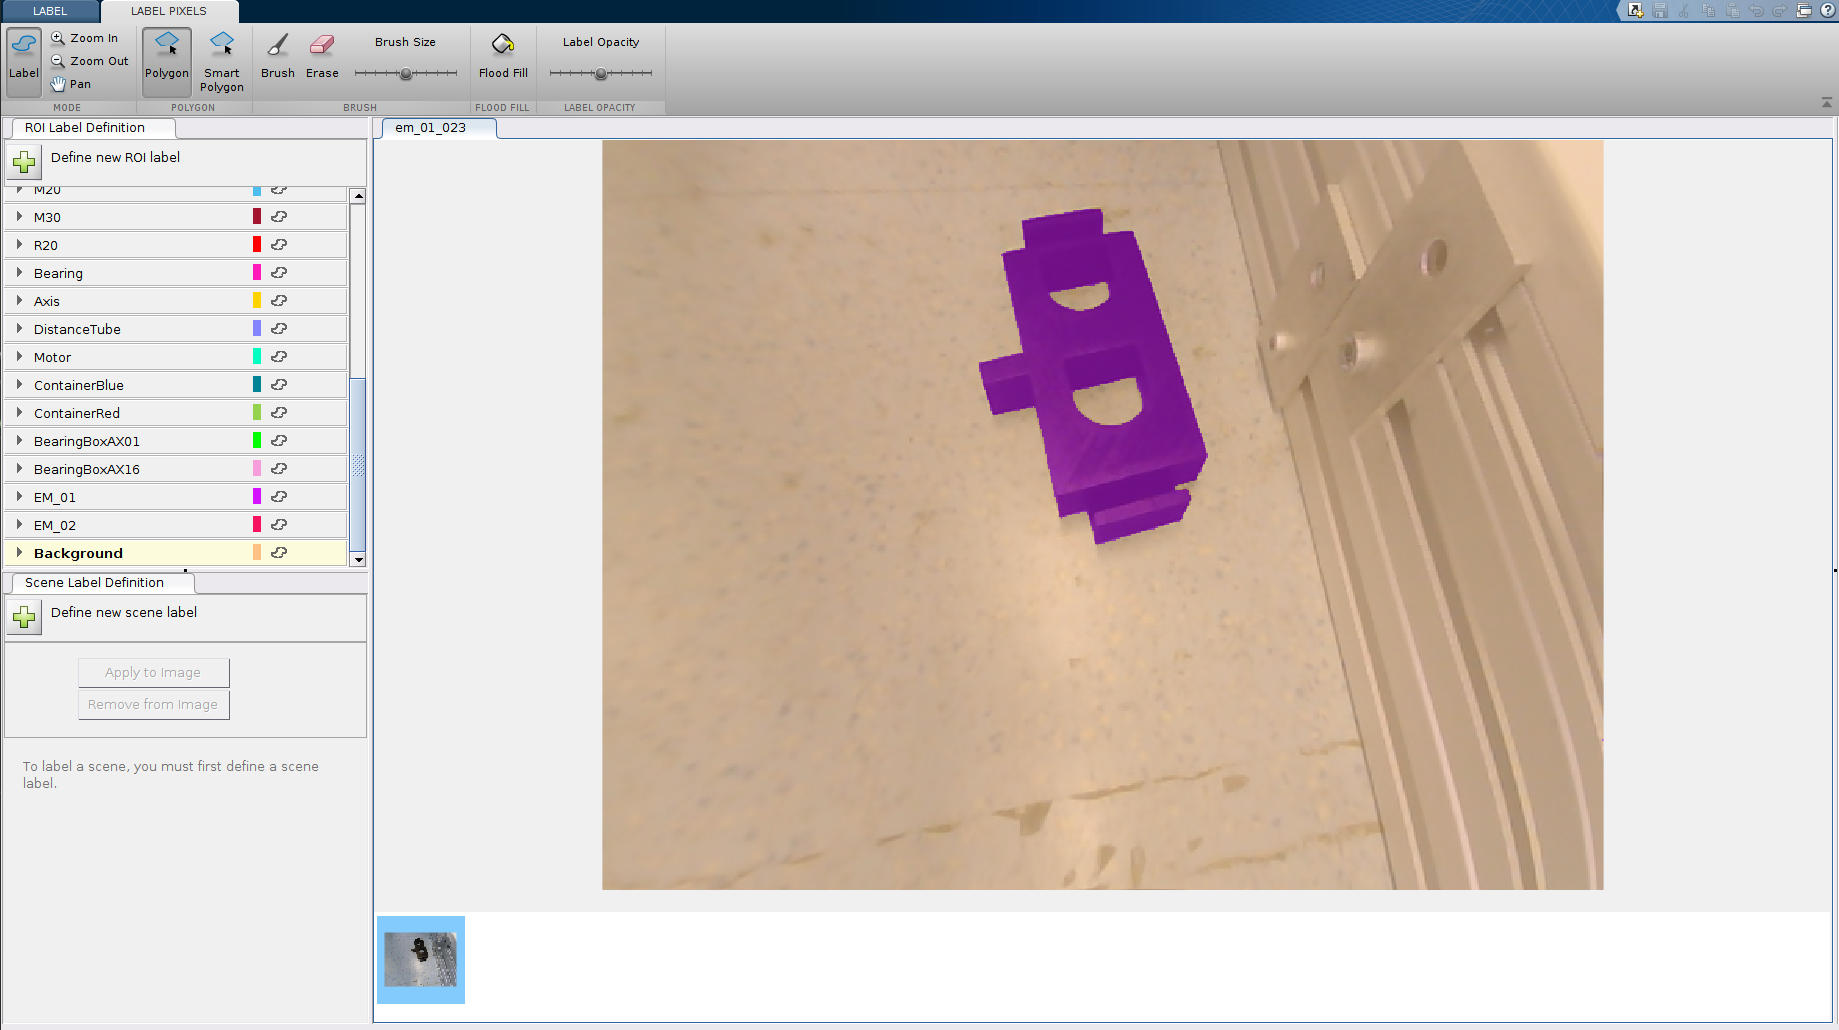
\includegraphics[width=.8\linewidth]{images/imglabler_eg}
		\captionsetup{justification=centering,margin=0.2cm}
		\caption{A sample object being labeled in ImageLabeler.}
		\label{Fig:annotate}
	\end{figure}

\end{frame}

\section{Artificial image generation}

\begin{frame}{Artificial image generation}

	\textbf{Motivation}
	\begin{small}
		\begin{itemize}
			\item For an image containing 1 desired object, roughly 4 minutes was spent for manual annotation.
			\item Capturing diverse real-world variations is time consuming.
		\end{itemize}
	\end{small}
		
	\vspace{5mm}
		
	\textbf{Process}
	\begin{small}
		\begin{itemize}
			\item Collect RGB intensity values of objects using manual annotation.
			\item Create a list of all the collected objects.
			\item For an artificial image, select a background image and random objects from the list of objects. 
			\item Place the selected objects at random locations and at random scales. 
			\item Correspondingly generate semantic labels and object detection labels.
		\end{itemize}
	\end{small}

\end{frame}

\begin{frame}{Artificial image generation}
	
	\textbf{Sample result}	
		
	\begin{figure}
		\centering
		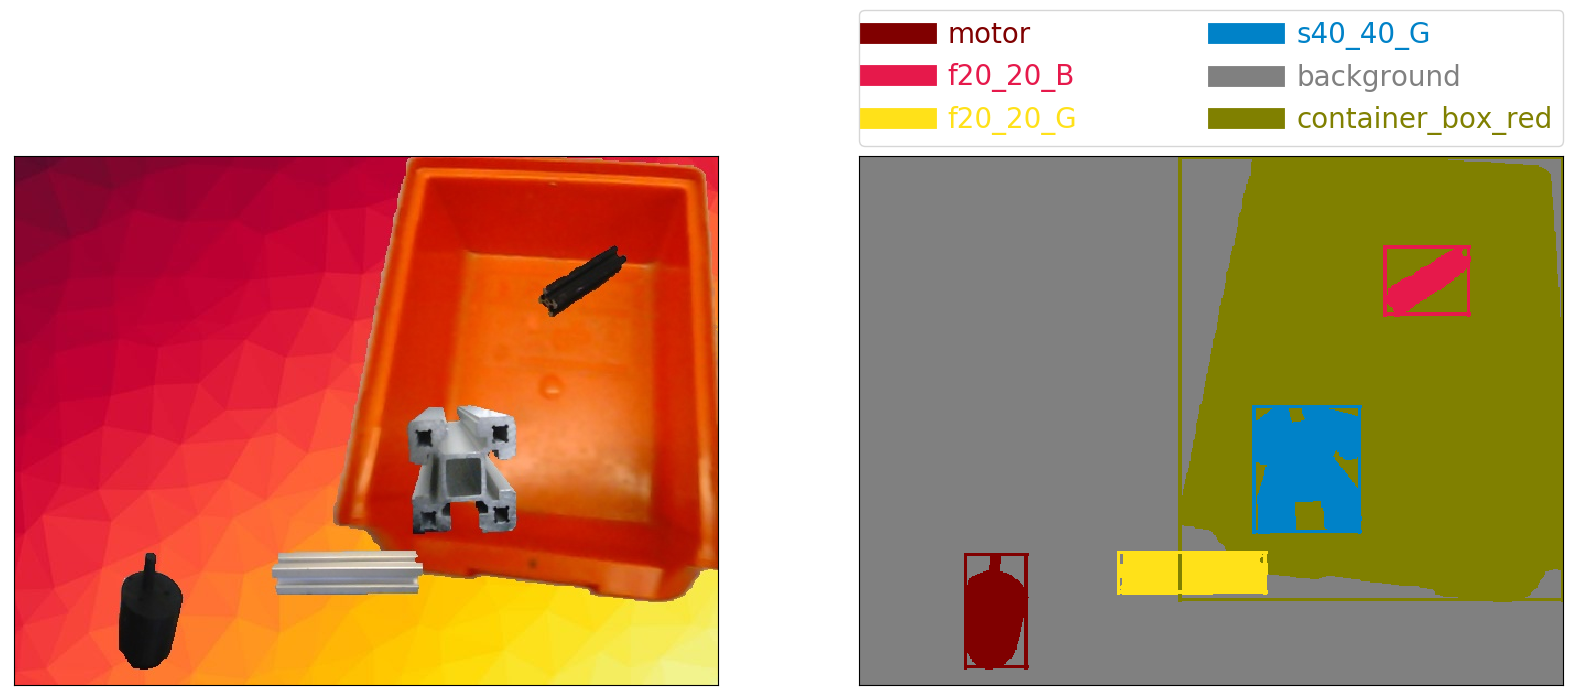
\includegraphics[scale=0.26]{images/sample_result_1}
		\captionsetup{justification=centering,margin=0.2cm}
		\caption{Sample results produced by the artificial image generation algorithm.}
		\label{Fig:sample}
	\end{figure}
\end{frame}

\section{Dataset variants}

\begin{frame}{Dataset variants}
\label{slide:motivvariants}

	\textbf{Motivation}
	\begin{small}
	
		\begin{itemize}
			\item Inability to distinguish size.
				\begin{figure}
				\centering
				\begin{subfigure}{.2\textwidth}
  					\centering
  					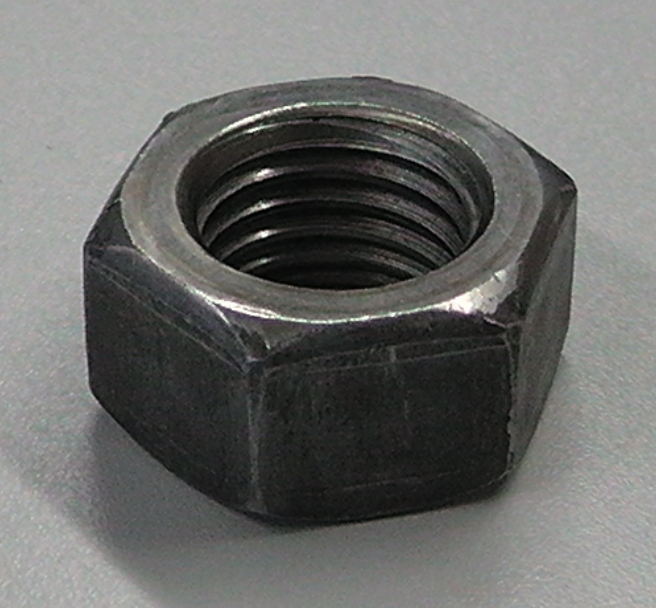
\includegraphics[width=.35\linewidth]{images/M20}
  					\caption{m20}
  					\label{Fig:size1}
				\end{subfigure}%
				\begin{subfigure}{.2\textwidth}
  					\centering
  					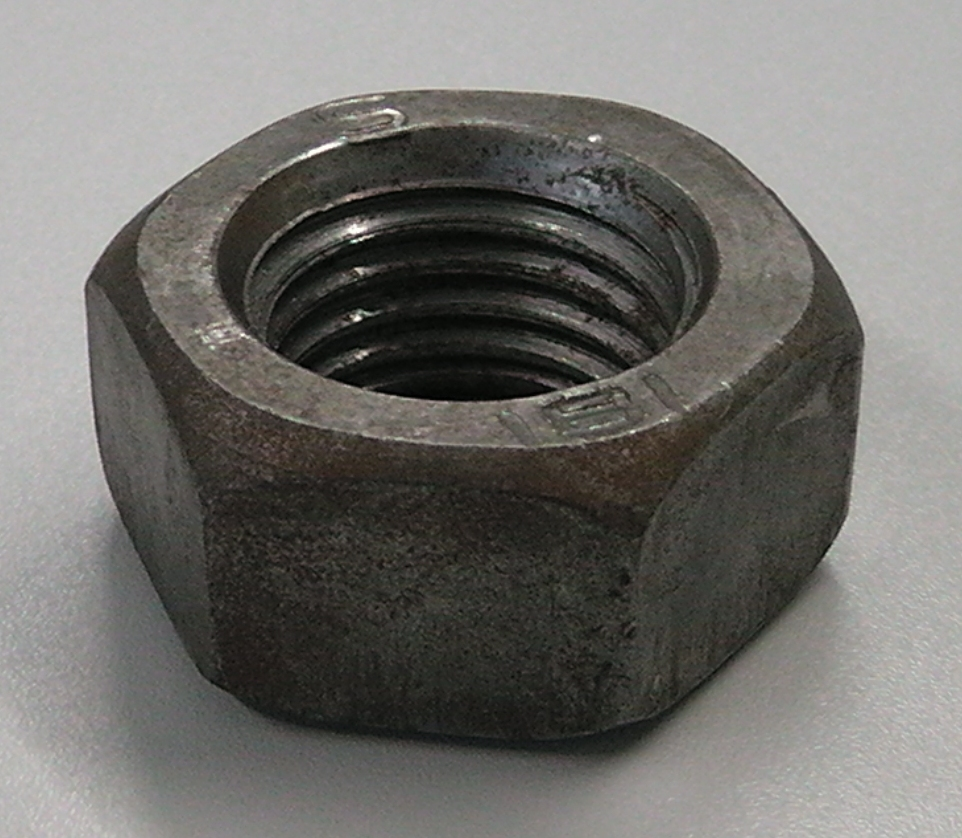
\includegraphics[width=.35\linewidth]{images/M30}
  					\caption{m30}
  					\label{Fig:size2}
				\end{subfigure}%
				\caption{m30 is larger than m20}
				\label{Fig:size}
				\end{figure}
				
			\item Inability to distinguish shape.
				\begin{figure}
				\centering
				\begin{subfigure}{.2\textwidth}
  					\centering
  					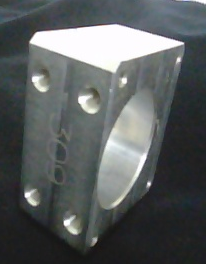
\includegraphics[width=.3\linewidth]{images/ax01_diff}
  					\caption{ax16}
  					\label{Fig:sim1a}
				\end{subfigure}%
				\begin{subfigure}{.2\textwidth}
  					\centering
  					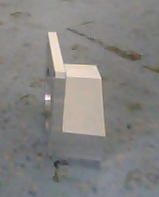
\includegraphics[width=.3\linewidth]{images/ax16_diff}
  					\caption{ax01}
  					\label{Fig:sim1b}
				\end{subfigure}%
				\begin{subfigure}{.23\textwidth}
  					\centering
  					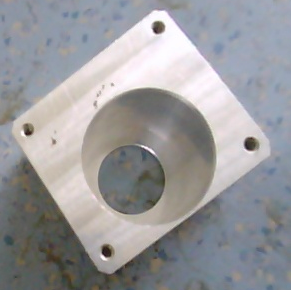
\includegraphics[width=.3\linewidth]{images/ax01_similar}
  					\caption{ax16}
  					\label{Fig:sim2a}
				\end{subfigure}%
				\begin{subfigure}{.21\textwidth}
  					\centering
  					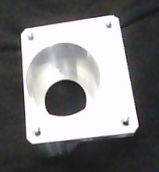
\includegraphics[width=.3\linewidth]{images/ax16_similar}
  					\caption{ax01}
  					\label{Fig:sim2b}
				\end{subfigure}%
				\caption{Bearing\_box ax16 and ax01 are distinguishable from similar viewpoints (a) and (b) but are indistinguishable from similar viewpoints (c) and (d).}
				\label{Fig:shape}
			\end{figure}
		\end{itemize}
			
	\end{small}

\end{frame}


\begin{frame}{Dataset variants}
	\textbf{Number of classes}
	\begin{small}
		\begin{table}
			\centering
			\begin{tabular}{|c|c|c|c|c|c|c|c|}
			\hline 
    		Variant & \makecell{Number of classes \\ including background} \\ 
			\hline 
			atWork\_full & 19 \\ 
			\hline 
			atWork\_size\_invariant & 15 \\ 
			\hline 
			atWork\_similar\_shapes & 13 \\ 
			\hline 
			atWork\_binary & 2 \\ 
			\hline 
			\end{tabular}
			\caption{Number of classes in dataset variants.}
			\label{Table:meta}
		\end{table}
	\end{small}
		
	\textbf{Number of images}
	\begin{small}	
		\begin{table}
			\centering
			\begin{tabular}{|c|c|c|c|c|c|c|c|}
			\hline 
    		& Training & Validation & Test \\ 
			\hline 
			Real Images & 396 & 72 & 69 \\ 
			\hline 
			Artificial Images & 7104 & 870 & 870 \\ 
			\hline 
			Total Images & 7500 & 942 & 939 \\ 
			\hline 
			\end{tabular}
			\caption{Number of images in the dataset.}
			\label{Table:meta}
		\end{table}
	\end{small}

\end{frame}

\section{Dataset analysis}

\begin{frame}{Dataset analysis}
\label{slide:analysis}
	\begin{small}
	\begin{itemize}
		\item Percentage of pixels of an object = $\frac{NP_o}{NP_s}$. \\
		$NP_o$ = Number of pixels occupied by the object in the training set. \\ $NP_s$ = Total number of pixels in the training set.
	\end{itemize}
	\begin{figure}
		\centering
		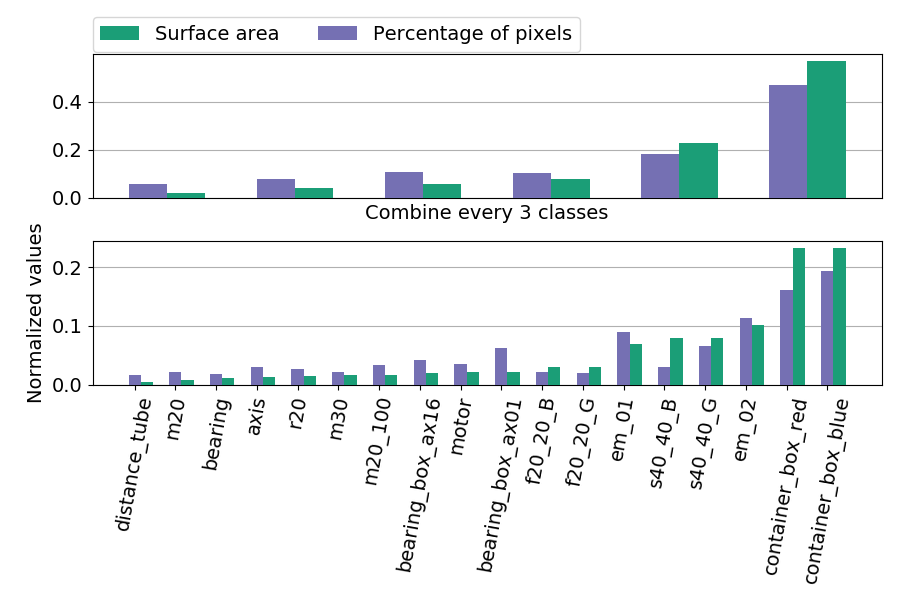
\includegraphics[scale=0.35]{images/analyzer_full}
		\captionsetup{justification=centering,margin=0.2cm}
		\caption{Percentage of pixels vs corresponding real-world surface area}
		\label{Fig:surarea}
	\end{figure}
	\end{small}

\end{frame}

\section{DeepLabv3+}

\begin{frame}{Architecture of DeepLabv3+}
	
	\begin{figure}
		\centering
		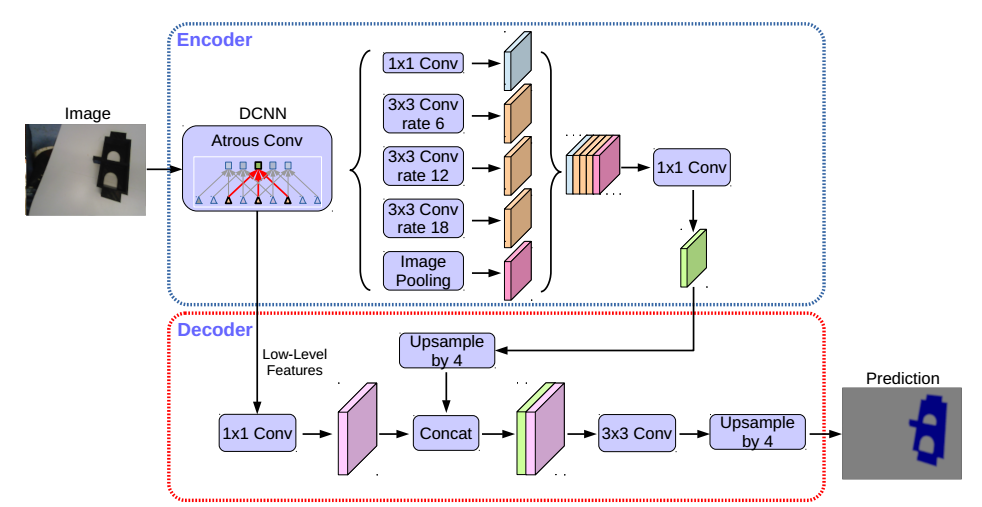
\includegraphics[width=1\linewidth]{images/deepLabv4}
		\captionsetup{justification=centering,margin=0.2cm}
		\caption{An illustration of DeepLabv3+ architecture. The encoder extracts features at different scales and the decoder refines object boundary delineation.}
		\label{Fig:deepLabv4}
	\end{figure}

\end{frame}


\begin{frame}{Depthwise seperable convolutions}
	\begin{small}
	\begin{itemize}
		\item First depthwise convolution, then pointwise convolution.
		\item Row 2 to row 5: depthwise convolution, 6th row: pointwise convolution.
	\end{itemize}
	\end{small}
	 
	\begin{figure}
		\centering
		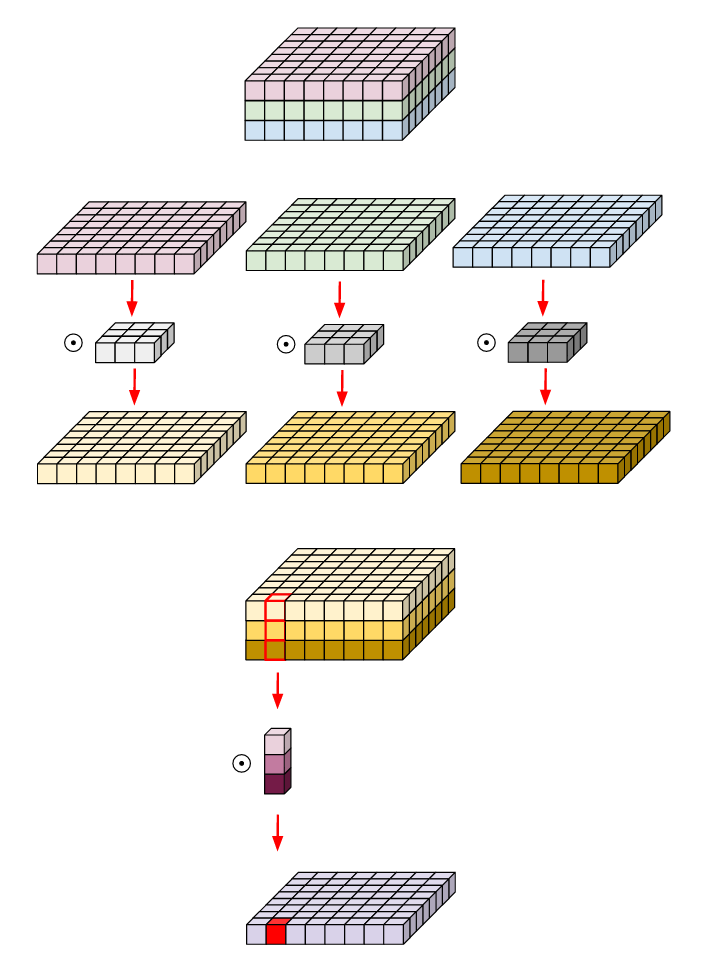
\includegraphics[width=.3\linewidth]{images/depthwise}
		\captionsetup{justification=centering,margin=0.2cm}
		\caption{Depthwise seperable convolution.}
		\label{Fig:depthwise}
	\end{figure}

\end{frame}

\begin{frame}{MobileNetv2 encoder of DeepLabv3+}
	\begin{small}
	\begin{itemize}
		\item Depthwise seperable convolutions.
		\item Inverted residual with linear bottleneck.
	\end{itemize}
	\end{small}
	
	\begin{figure}
		\centering
		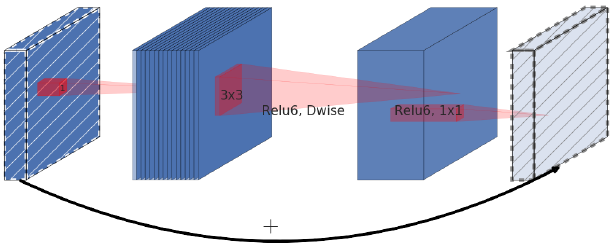
\includegraphics[width=.6\linewidth]{images/inverted_residual}
		\captionsetup{justification=centering,margin=0.2cm}
		\caption{Inverted residual block}
		\label{Fig:residual}
	\end{figure}

\end{frame}

\begin{frame}{Xception encoder of DeepLabv3+}

	\begin{figure}[h]
		\centering
		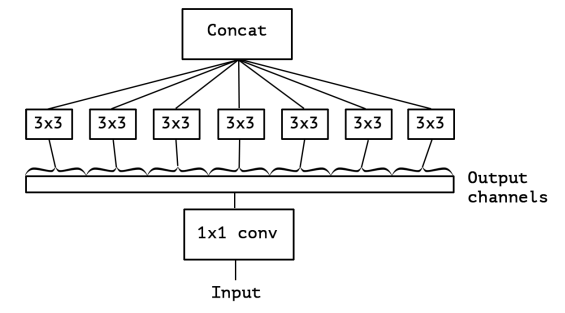
\includegraphics[width=0.5\linewidth]{images/extreme_inception}
		\captionsetup{justification=centering,margin=0.2cm}
		\caption{Xception module}
		\label{Fig:xception}
	\end{figure}

\end{frame}

\begin{frame}{Atrous separable convolutions}


\end{frame}

\section{Results}

\begin{frame}{Comparing encoders}
	\begin{small}
		\begin{itemize}
			\item 
		Per class IOU = $\frac{ground\_truth \: \cap \: prediction}{ground\_truth \: \cup \: prediction}$
			\item mIOU = mean of all class IOUs.
			\item DeepLabv3+ with Xception encoder achieves higher mIOU on all four dataset variants.
		\end{itemize}
	
		\begin{table}[h]
			\begin{tabular}{|l|r|r|}
			\hline
			\multicolumn{ 1}{|l|}{\makecell{\textbf{Dataset variant}}} & \multicolumn{ 2}{l|}{\makecell{\textbf{mIOU in \%}}} \\ \cline{ 2- 3}
			\multicolumn{ 1}{|l|}{} & \multicolumn{1}{l|}{MobileNetv2} & 			\multicolumn{1}{l|}{Xception} \\ \hline
			atWork\_full & 77.47 & 89.63 \\ \hline
			atWork\_size\_invariant & 83.10 & 92.47 \\ \hline
			atWork\_similar\_shapes & 82.10 & 90.71 \\ \hline
			atWork\_binary & 96.06 & 98.68 \\ \hline
			\end{tabular}
			\captionsetup{justification=centering,margin=2cm}
			\caption{This table lists the mIOU obtained by DeepLabv3+ with MobileNetv2 and Xception encoders on 4 dataset variants.} 
			\label{Table:vars}
		\end{table}
	\end{small}

\end{frame}

\begin{frame}{Comparing dataset variants}
	\begin{small}
		\begin{itemize}
			\item Background/foreground segmentation leads to the highest mIOU.
			\item Treating all objects as different classes leads to the lowest mIOU.
			\item Combining objects similar in shape, size or color improves mIOU.
		\end{itemize}
	\end{small}
	
	\begin{figure}[h]
		\centering
		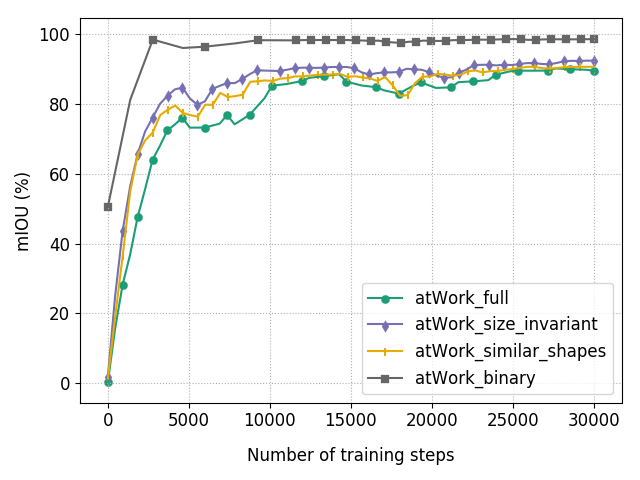
\includegraphics[width=0.4\linewidth]{images/xcep_4vars}
		\captionsetup{justification=centering,margin=2cm}
		\caption{mIOU (\%) vs Number of training steps \\ DeepLabv3+ with Xception encoder on all dataset variants}
		\label{Fig:variants}
	\end{figure}

\end{frame}


%\begin{frame}{Training with different data}
%
%
%\end{frame}


\begin{frame}{Comparing individual classes}

	\begin{small}
		\begin{itemize}
			\item 9.88 \% of pixels belonging to m30 is classified as m20. 
			\item 9.97 \% of pixels belonging to bearing box ax16 is classified as bearing box ax01 [Slide \ref{slide:motivvariants}].
		\end{itemize}
	\end{small}		
	
	\begin{figure}[h]
		\centering
		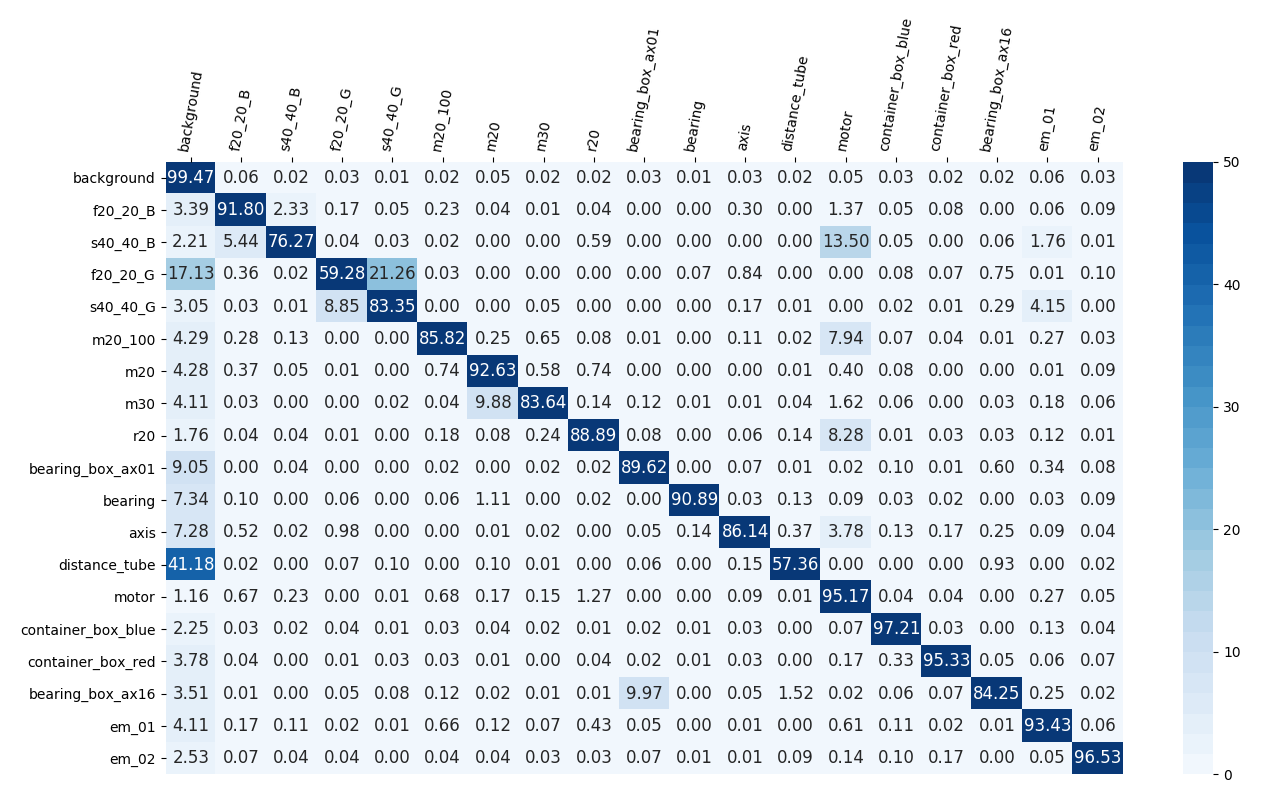
\includegraphics[width=0.65\linewidth]{images/cm_full}
		\captionsetup{justification=centering,margin=0.2cm}
		\caption{Confusion matrix on atWork\_full dataset variant by DeepLabv3+ with MobileNetv2 encoder.}
		\label{Fig:variants}
	\end{figure}

\end{frame}

\begin{frame}{Comparing individual classes}
	\begin{small}
		\begin{itemize}
			\item Class IOU shows an increasing trend with increase in Percentage of pixels.
			\item Percentage of pixels is shown to increase with surface area [Slide \ref{slide:analysis}].
		\	item DeepLabv3+ tends to learn larger objects first.
		\end{itemize}
	\end{small}

	\begin{figure}[h]
		\centering
		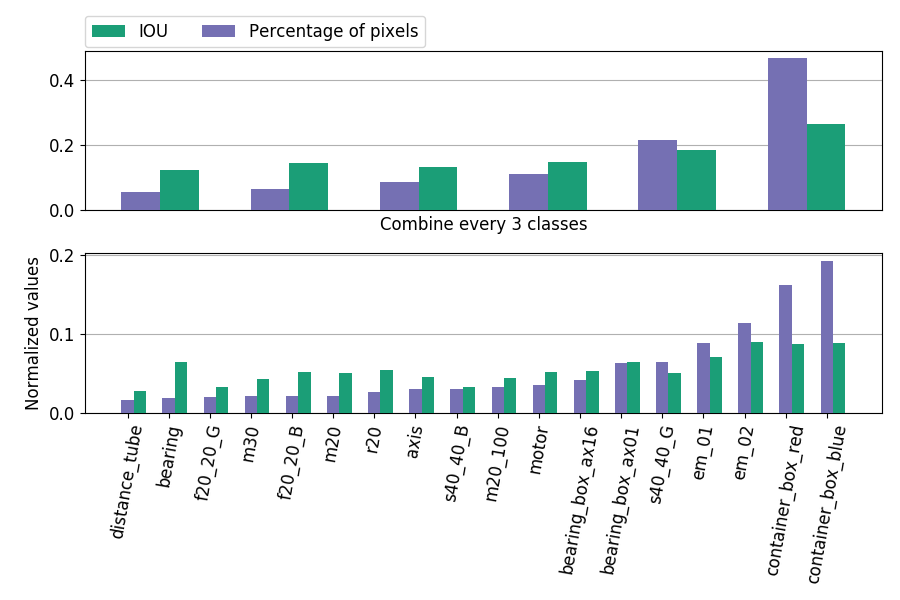
\includegraphics[width=0.57\linewidth]{images/cls_iou_full}
		\captionsetup{justification=centering,margin=0.2cm}
		\caption{Individual class IOUs achieved by DeepLabv3+ with MobileNetv2 encoder is plotted with the percentage of pixels.}
		\label{Fig:variants}
	\end{figure}

\end{frame}


\begin{frame}{Quantizing the inference graph}
	\begin{small}
		\begin{itemize}
			\item The inference graph is quantized.
			\item With MobileNetv2 encoder, 67 \% drop in occupied disk memory is achieved. Drop in mIOU is around 9 \%.
			\item With Xception encoder, 73 \% drop in occupied disk memory is achieved. Drop in mIOU is around 2 \%.
		\end{itemize}
	\end{small}
	
	
\end{frame}

\begin{frame}{Quantizing the inference graph}
	\begin{small}
		\begin{table}[h]
			\centering
			\begin{tabular}{|l|l|l|l|l|}
			\hline
			\makecell{\textbf{Encoder}} & \makecell{\textbf{mIOU} \\ \textbf{(\%)}} & \makecell{\textbf{Number of} \\ \textbf{parameters}} & \makecell{\textbf{FLOPS}} & \makecell{\textbf{Disk memory} \\ \textbf{(MB)}} \\ \hline
			MobileNetv2 & 84.66 & 2.11M & 6.41B & 8.7 \\ \hline
			MobileNetv2-8 & 75.17 & 2.11M & 328.87M & 2.8 \\ \hline
			Xception & 92.42 & 41.05M & 126.27B & 165.6 \\ \hline
			Xception-8 & 90.4 & 41.05M & 1.94B & 44.7 \\ \hline
			\end{tabular}
			\captionsetup{justification=centering,margin=0.2cm}
			\caption{This table summarizes the average mIOU across all four dataset variants, number of parameters, and floating point operations (FLOPS) of both the quantized and full precision encoders of DeepLabv3+. "M" denotes million and "B" denotes billion.}
			\label{Table:quantMetrics}
		\end{table}	
	\end{small}

\end{frame}


\section{Contributions and future work}

\begin{frame}{Conclusion and future work}
\textbf{Contributions}
	\begin{small}
		\begin{itemize}
			\item Artificial image generation algorithm.
			\item Segmentation dataset with 18 atWork objects.
			\item Evaluation of DeepLabv3+ with resource efficient encoders MobileNetv2 and Xception.
		\end{itemize}
	\end{small}
	
\vspace{5mm}
\textbf{Future work}
	\begin{small}
		\begin{itemize}
			\item Model interpretability.
			\item Architecture search.
			\item Fusion of 2D image data with point cloud information.
		\end{itemize}
	\end{small}

\end{frame}


\begin{frame}{Thank you very much!}
\usebeamerfont{AAA}
Are there any questions? \\
\end{frame}

\begin{frame}
  \frametitle{References}
  \printbibliography[title={References}]	
\end{frame}

\end{document}
